\documentclass[paper=a4, fontsize=11pt]{article} % A4 paper and 11pt font size
\usepackage[a4paper, margin=1.3in]{geometry}
% ---- Entrada y salida de texto -----

\usepackage[T1]{fontenc} % Use 8-bit encoding that has 256 glyphs
\usepackage[utf8]{inputenc}
% \usepackage[light,math]{iwona}

\usepackage{fancyhdr}
\usepackage{fancybox}
\usepackage{pseudocode}


% ---- Idioma --------

\usepackage[spanish, es-tabla]{babel} % Selecciona el español para palabras introducidas automáticamente, p.ej. "septiembre" en la fecha y especifica que se use la palabra Tabla en vez de Cuadro

% ---- Otros paquetes ----

\usepackage{amsmath,amsfonts,amsthm} % Math packages
\usepackage{graphics,graphicx, floatrow} %para incluir imágenes y notas en las imágenes
\usepackage{graphics,graphicx, float} %para incluir imágenes y colocarlas
\usepackage{enumerate}
\usepackage{subfigure}
% \makesavenoteenv{tabular}
% \makesavenoteenv{table}
% Para hacer tablas comlejas
%\usepackage{multirow}
%\usepackage{threeparttable}
\usepackage{sectsty} % Allows customizing section commands
\allsectionsfont{\centering \scshape} % Make all sections centered, the default font and small caps

\usepackage{fancyhdr} % Custom headers and footers
\usepackage[usenames, dvipsnames]{color}
\usepackage{colortbl}
% \usepackage{minted}
\usepackage{xcolor}
\usepackage{url}
\usepackage{cancel}

% \newmintedfile[mycpp]{c++}{
%     linenos,
%     numbersep=5pt,
%     gobble=0,
%     frame=lines,
%     framesep=2mm,
% }

% \newmintedfile[myc]{c}{
%     linenos,
%     numbersep=5pt,
%     gobble=0,
%     frame=lines,
%     framesep=2mm,
% }

% \newmintedfile[mypython]{python}{
%     linenos,
%     numbersep=5pt,
%     gobble=0,
%     frame=lines,
%     framesep=2mm,
% }

\usepackage{cite}

\usepackage[bookmarks=true,
    bookmarksnumbered=false, % true means bookmarks in
             % left window are numbered
    bookmarksopen=false,   % true means only level 1
             % are displayed.
    colorlinks=true,
    urlcolor=webblue,
    citecolor=webred,
    linkcolor=webblue]{hyperref}
\definecolor{webgreen}{rgb}{0, 0.5, 0} % less intense green
\definecolor{webblue}{rgb}{0, 0, 0.5}  % less intense blue
\definecolor{webred}{rgb}{0.5, 0, 0} % less intense red

%% Define a new 'leo' style for the package that will use a smaller font.
\makeatletter
\def\url@leostyle{%
  \@ifundefined{selectfont}{\def\UrlFont{\sf}}{\def\UrlFont{\small\ttfamily}}}
\makeatother
%% Now actually use the newly defined style.
\urlstyle{leo}

\pagestyle{fancyplain} % Makes all pages in the document conform to the custom headers and footers
\fancyhead{} % No page header - if you want one, create it in the same way as the footers below
\fancyfoot[L]{} % Empty left footer
\fancyfoot[C]{} % Empty center footer
\fancyfoot[R]{\thepage} % Page numbering for right footer
\renewcommand{\headrulewidth}{0pt} % Remove header underlines
\renewcommand{\footrulewidth}{0pt} % Remove footer underlines
\setlength{\headheight}{13.6pt} % Customize the height of the header

\numberwithin{equation}{section} % Number equations within sections (i.e. 1.1, 1.2, 2.1, 2.2 instead of 1, 2, 3, 4)
\numberwithin{figure}{section} % Number figures within sections (i.e. 1.1, 1.2, 2.1, 2.2 instead of 1, 2, 3, 4)
\numberwithin{table}{section} % Number tables within sections (i.e. 1.1, 1.2, 2.1, 2.2 instead of 1, 2, 3, 4)

\setlength\parindent{0pt} % Removes all indentation from paragraphs - comment this line for an assignment with lots of text

\newcommand{\horrule}[1]{\rule{\linewidth}{#1}} % Create horizontal rule command with 1 argument of height

%%%%% Para cambiar el tipo de letra en el título de la sección %%%%%%%%%%%
% \usepackage{sectsty}
% \chapterfont{\fontfamily{pag}\selectfont} %% for chapter if you want
% \sectionfont{\fontfamily{pag}\selectfont}
% \subsectionfont{\fontfamily{pag}\selectfont}
% \subsubsectionfont{\fontfamily{pag}\selectfont}

%----------------------------------------------------------------------------------------
% TÍTULO Y DATOS DEL ALUMNO
%----------------------------------------------------------------------------------------

\title{
\normalfont \normalsize
\textsc{{\bf Redes y Sistemas Complejos (2016-2017)} \\ Grado en Ingeniería Informática \\ Universidad de Granada} \\ [25pt] % Your university, school and/or department name(s)
\horrule{0.5pt} \\[0.4cm] % Thin top horizontal rule
\huge Memoria Práctica 4\\ Estudio de la red de amistad en Twitter de Python Granada para el aumento de la difusión de las publicaciones a lo largo de las distintas comunidades que la rodean.\\% The assignment title
\horrule{2pt} \\[0.5cm] % Thick bottom horizontal rule
}

\author{Braulio Vargas López\\DNI: 20079894C\\Correo: brauliovarlop@correo.ugr.es} % Nombre y apellidos

\date{\normalsize\today} % Incluye la fecha actual

%----------------------------------------------------------------------------------------
% DOCUMENTO
%----------------------------------------------------------------------------------------

\begin{document}

\maketitle % Muestra el Título
\pagenumbering{gobble}
\newpage %inserta un salto de página

\tableofcontents % para generar el índice de contenidos
\newpage
\pagenumbering{arabic}

\section{Definición del problema, selección del dominio y obtención de los datos.}

\subsection{Definición del problema}

Hace unos años, surgió en Granada la comunidad de Python, para que gente que programase en este lenguaje, quisiera aprenderlo, preguntar dudas, etc. y dar visibilidad a los programadores de Python que había en Granada. Durante un tiempo la comunidad funcionó bien, tanto por redes sociales, como comunidad física, pero su actividad cesó y quedó, por así decirlo, muerta.

El año pasado, la comunidad de \textit{\textbf{Python Granada}} se reactivó y comenzó de nuevo su actividad, tanto con eventos, como fue el ``\textit{PyDay}'', como su actividad como comunidad en redes sociales como en \href{https://twitter.com/python_granada}{Twitter} y \href{https://www.facebook.com/Pythongranada/?fref=ts}{Facebook}, y en el grupo de \href{https://t.me/pythongranada}{Telegram}.

Durante el tiempo que estuvimos organizando el ``renacer'' de la comunidad, yo me ofrecí a llevar la cuenta de Python Granada y pude observar cómo poco a poco iba creciendo el número de usuarios a los que llegábamos y cómo cada vez teníamos más relaciones con cuentas relacionadas con Python. A raíz de esto vienen las preguntas a resolver en este estudio:
\begin{enumerate}[$\bullet$]
    \item \textbf{¿Qué comunidades existen en el entorno más cercano de Python Granada en Twitter y a qué usuarios llega?}
    \item \textbf{¿Cuál es la influencia en esta red de Python Granada?}
\end{enumerate}

\subsection{Selección del dominio}

El dominio en el que se mueve el problema, será una red dirigida de usuarios de la red social \textit{Twitter}, donde los nodos son los propios usuarios de Twitter que se encuentran en la red cercana a la cuenta de Python Granada y los enlaces marcan la relación \textit{Siguiendo $\iff$ Seguidor} entre los usuarios. Los usuarios que vamos almacenando tienen una relación de amistad, es decir que el usuario $x_i$ tiene un conjunto de amigos $F$, donde a cada $F_i$ es seguido por el usuario $x_i$.

Estos enlaces tendrán una ponderación igual a 1, ya que inicialmente no conocemos nada del peso que puede tener un enlace entre dos nodos.

\subsection{Obtención de los datos}

Para obtener los datos de Twitter, se ha usado la biblioteca \href{http://www.tweepy.org/}{Tweepy} para conectarnos a Twitter haciendo uso de Python. Para obtener los datos de Twitter, es necesario generar una nueva app para poder obtener las claves y tokens de acceso para poder extraer los datos que vamos a utilizar. Una vez hecho, haciendo uso de Django y SQLite, tenemos un \textit{crawler} de usuarios en Twitter, que va recorriendo usuarios en función de la amistad y almacenándolos en una base de datos SQLite, para poder trabajar más tranquilamente con la red.

Tras recorrer la lista completa de amistad de la cuenta de Python Granada, habrá almacenados más de 30000 usuarios y más de 42000 enlaces, que representan la red de amistad más cercana. Esta red es dirigida, ya que un usuario $x$ puede estar siguiendo $y$, pero puede que el usuario $y$ no siga al usuario $x$.

\section{Medidas estudiadas de la red}

Las medidas extraídas de la red podemos verlas de forma resumida a continuación:
\begin{table}[H]
\begin{tabular}{|l|r|}
  \hline
  Medida & Valor \\
  \hline
  Número de nodos & 31293 \\
  \hline
  Número de enlaces & 42487 \\
  \hline
  Grado medio & 2.715 \\
  \hline
  Grado medio con pesos & 1.358 \\
  \hline
  Longitud media del camino & 2.895 \\
  \hline
  Diámetro de la red & 5 \\
  \hline
  Densidad de grafo & 0 \\
  \hline
  Modularidad & 0.743 \\
  \hline
  Componentes conexas & 55\\
  \hline
  Coef. de clustering & 0.103\\
  \hline
\end{tabular}
\label{estadisticas}
\caption{Principales medidas estadísticas extraídas de la red.}
\end{table}

Esto es un pequeño y visual resumen de las principales medidas estadísticas obtenidas de la red, pero, ahora vamos a verlas con más detalle.

\subsection{Grado medio y grado medio con pesos}

Como hemos podido ver en la \hyperref[estadisticas]{Tabla \ref*{estadisticas}}, el grado medio y el grado medio con pesos es muy bajo. A priori, sin mirar ningún nodo de la red, podría parecer que el grado de los nodos de la red son bajos, pero si nos fijamos en estos, podremos ver que existen nodos con grado 4628, nodos con casi grado 3000, etc. por lo que la medida del grado medio no es muy representativa de la red. Aunque sí indica que existe un gran número de nodos con un grado pequeño, como podemos ver en la \hyperref[im1]{Figura \ref*{im1}}.

\begin{figure}[H]
    \centering
    \mbox {
        \subfigure[Distribución de grados.]{
        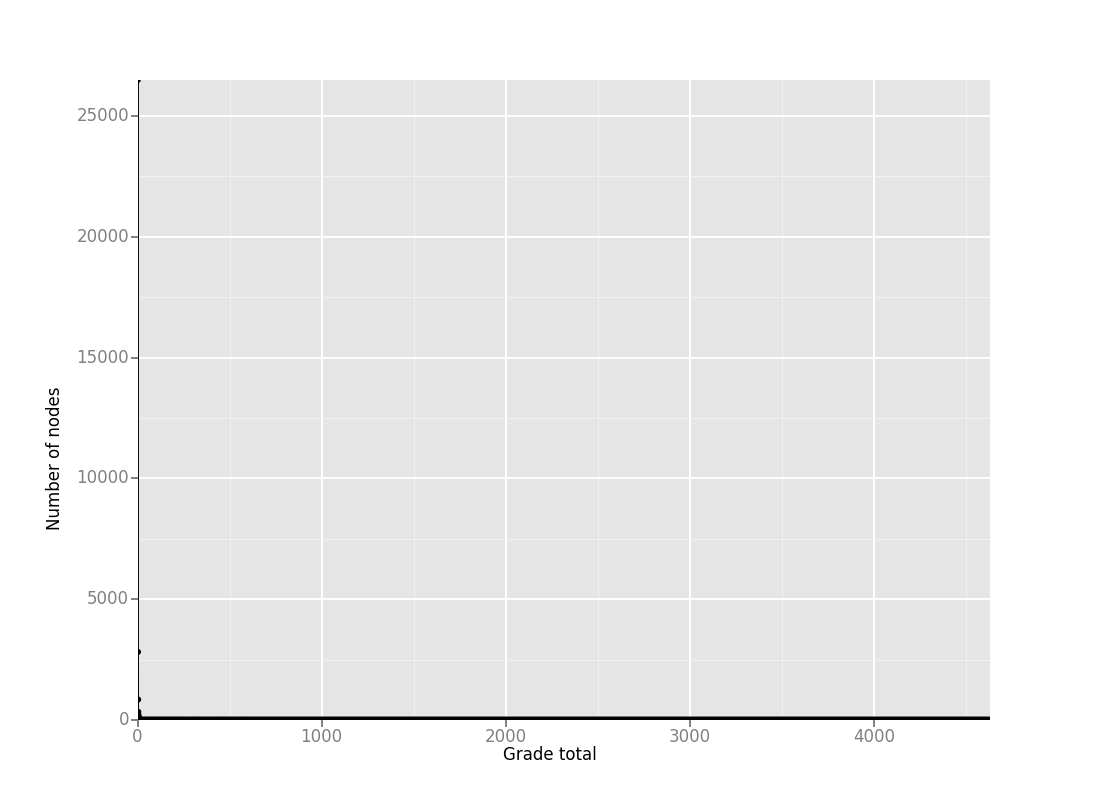
\includegraphics[width=0.5\textwidth]{img/dist_hist_total}
        \label{im1tot}
        }
    }
    \mbox{
        \subfigure[Distribución de grados de entrada.] {
            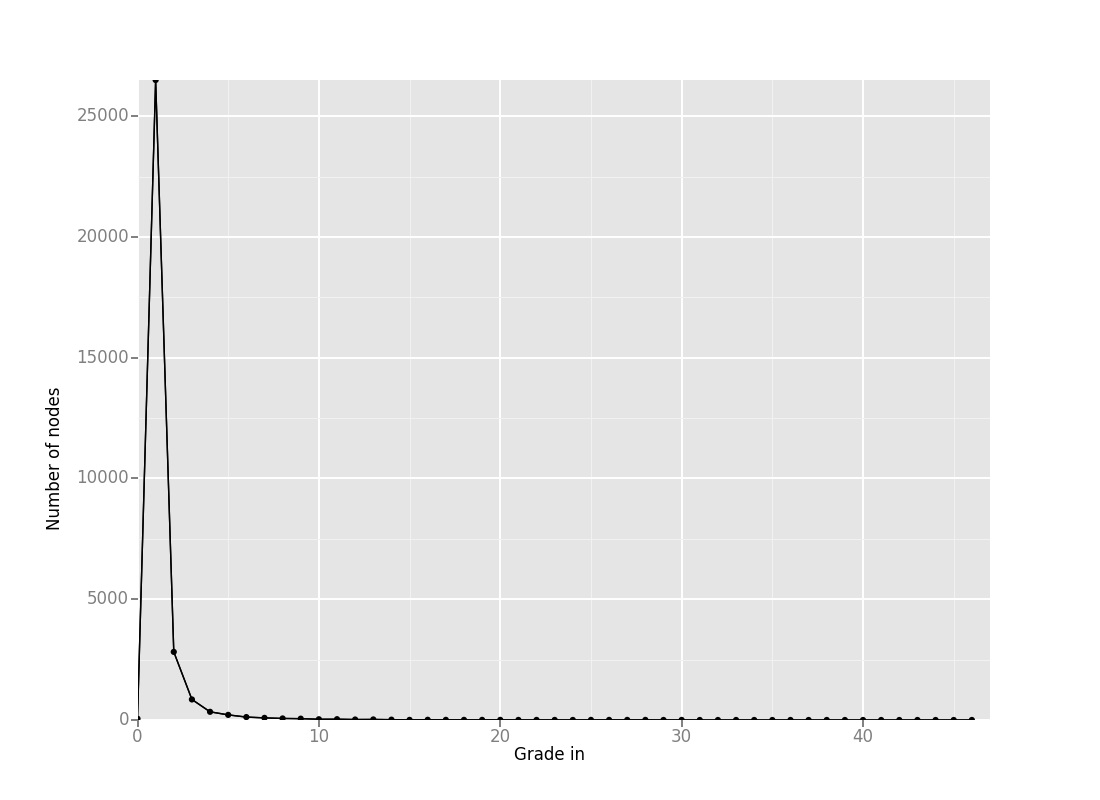
\includegraphics[width=0.5\textwidth]{img/dist_hist_in}
            \label{im1in}
        }
        \qquad
        \subfigure[Distribución de grados de salida.] {
            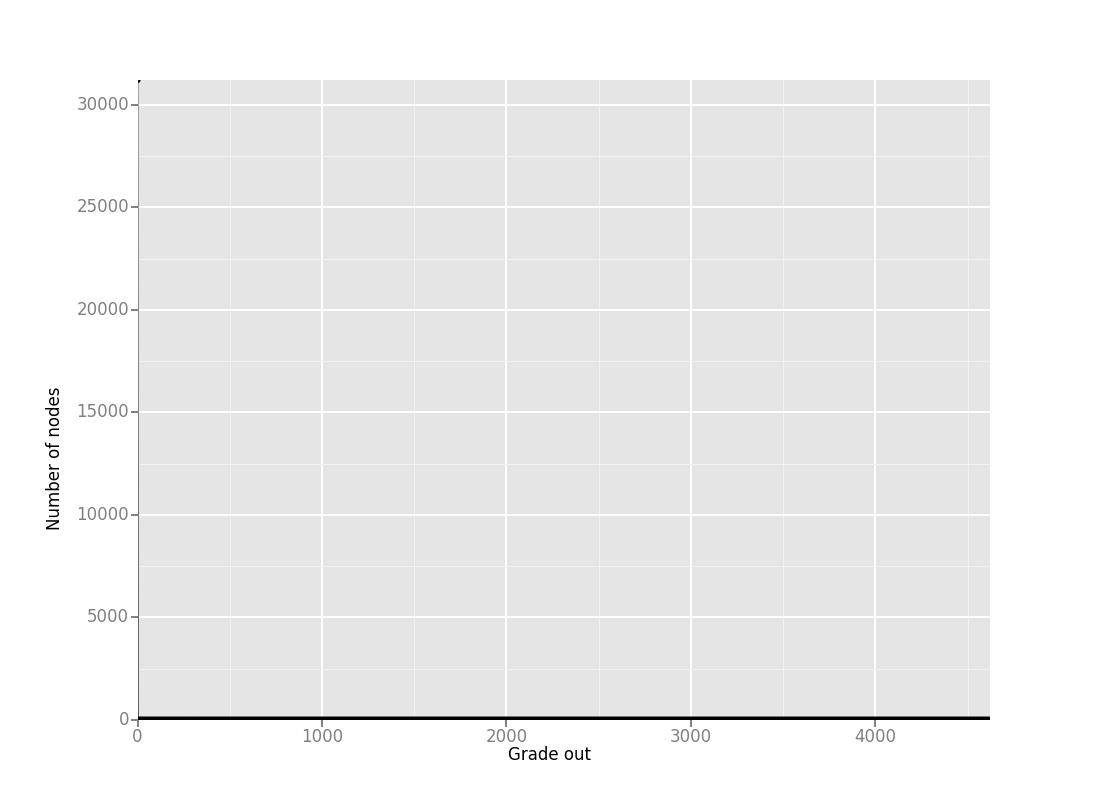
\includegraphics[width=0.5\textwidth]{img/dist_hist_out}
            \label{im1out}
        }
    }
    \caption{Gráficas de distribución de grados.}
    \label{im1}
\end{figure}

\subsection{Longitud del camino medio y diámetro de la red}

La longitud media del camino, nos indica que en media, podemos llegar desde cualquier nodo a otro diferente en 2.895 pasos y el diámetro de la red nos indica la longitud del camino mínimo más largo. En este caso, el camino mínimo más largo para llegar desde un nodo $X$ a un nodo $Y$ es de 5 pasos. Esto nos indica la presencia de hubs en la red que acortan mucho las distancias entre los nodos. En la \hyperref[im2]{Figura \ref*{im2}}, podemos ver la distribución de distancias de la red.

\begin{figure}[H]
  \centering
  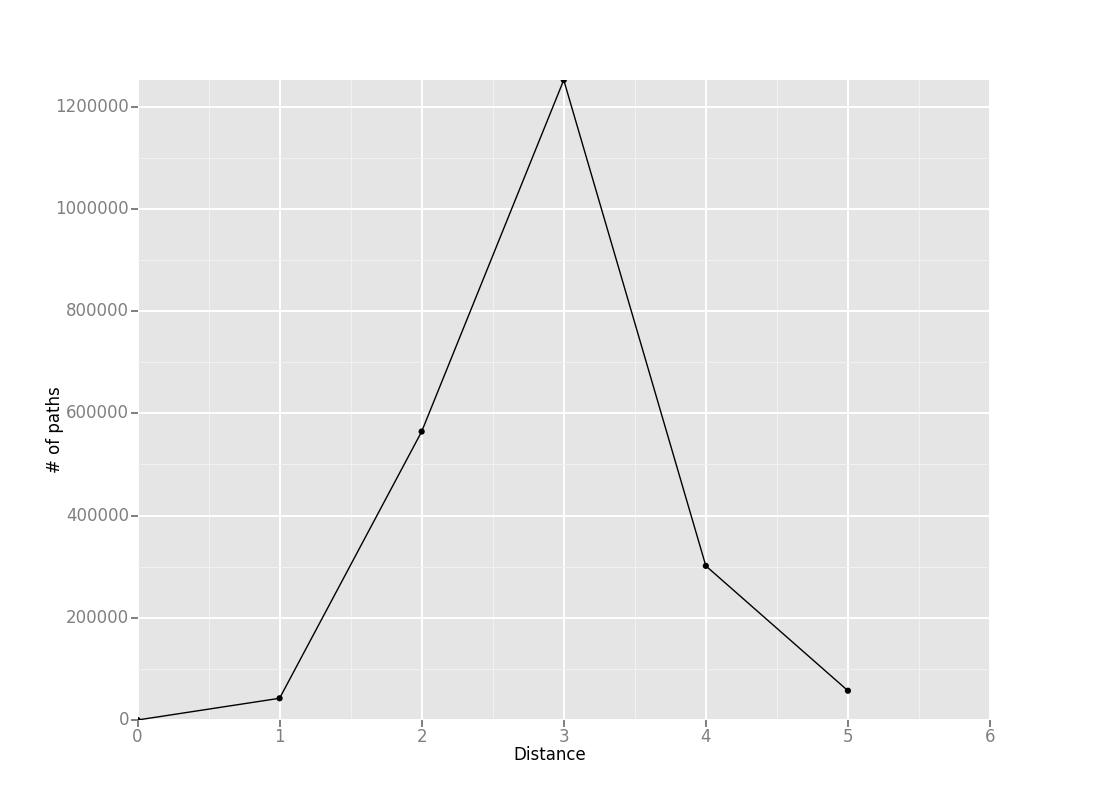
\includegraphics[width=0.7\textwidth]{img/dist_hist}
  \caption{Distribución de distancias de la red.}
  \label{im2}
\end{figure}

Como podemos ver en la gráfica, el pico que existe en torno a la distancia 3, significa que la mayoría de los nodos tienen una distancia igual a la media, 2.895, siendo el camino mínimo de mayor longitud 5, que es el diámetro de la red.

\subsection{Densidad de la red}

El número de nodos en esta red es de 31923 y 42487 aristas, de los $\frac{n(n-1)}{2}$ nodos posibles. Para calcular la densidad de la red se usa la siguiente fórmula:
\begin{displaymath}
    D = \frac{L}{L_{max}} = \frac{L}{\frac{n(n-1)}{2}} = \frac{42487}{\frac{31293\cdot31292}{2}} = 8.6777\cdot10^{-5} \approx 0
\end{displaymath}

De aquí viene que el valor de la densidad que podemos ver en la \hyperref[estadisticas]{Tabla \ref*{estadisticas}} sea 0, y es que tiene muy pocos enlaces en comparación con los enlaces totales que podía tener, por lo que la red es muy poco densa, tanto que su densidad tiende a 0.

\subsection{Coeficiente de clustering y modularidad}

El coeficiente de clustering global, nos indica la probabilidad que existe en que dados dos nodos $n_i$ y $n_k$ escogidos aleatoriamente de la red estén conectados entre sí. Se calcula como la suma de los coeficientes de clustering locales de todos los nodos de la red:

\begin{displaymath}
    C_i = \frac{2L_i}{k_i(k_i - 1)} \Longrightarrow <C> = \frac{1}{N}\sum_{i=1}^NC_i
\end{displaymath}

En este caso, el coeficiente de clustering es de 0.103, que lo que nos indica que para el tamaño de la red, el coeficiente de clustering es siginificativo y nos indica que existe un cierto nivel de transitividad en la red, es decir, que los amigos de un nodo es bastante probable que también estén conectados entre sí. Esto lo podemos ver representado en la \hyperref[im3]{Figura \ref*{im3}}.

\begin{figure}[H]
  \centering
  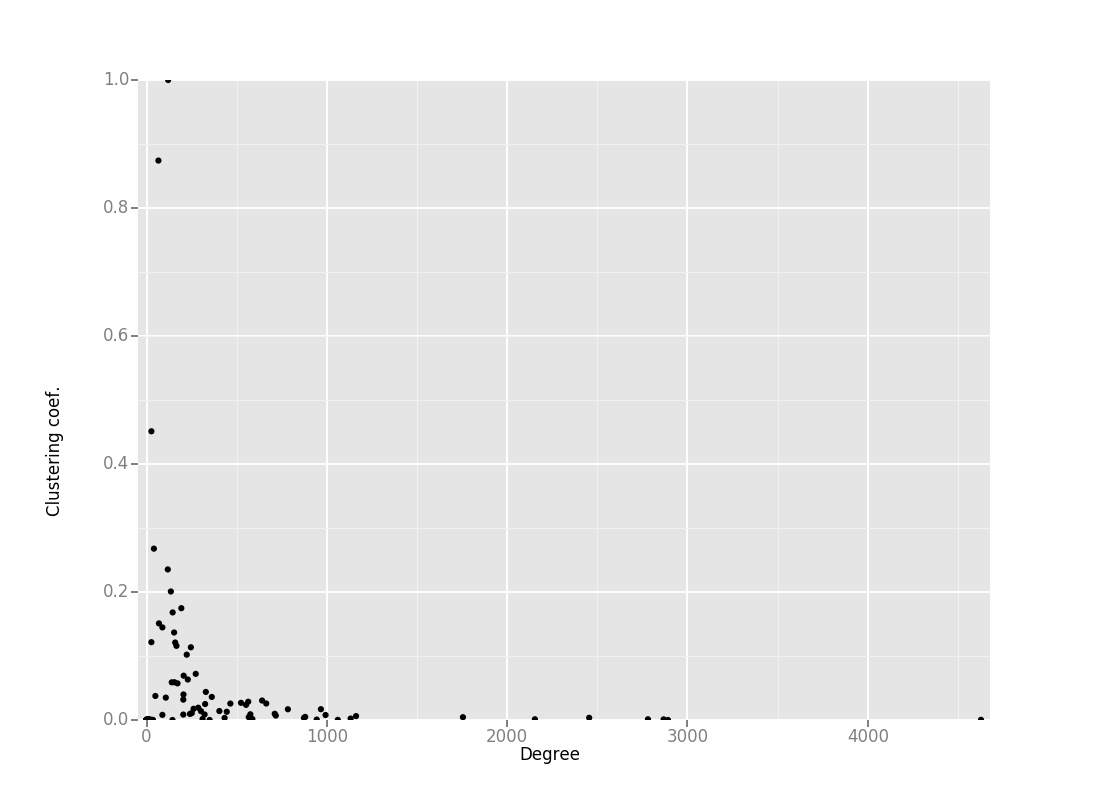
\includegraphics[width=0.7\textwidth]{img/clust_hist}
  \caption{Histograma del coeficiente de clustering.}
  \label{im3}
\end{figure}

Con esto pasamos al coeficiente de modularidad. La modularidad nos indica si la red tiene una estructura modular interna que sea coherente, es decir, que dentro de la red existen una serie de comunidades con un menor número de enlaces entre estas menor del que habría en una red aleatoria equivalente. Además, también indica cómo de buena es la partición en comunidades que hemos realizado. Este valor $Q$ oscila en el intervalo $[-1,1]$, siendo mejor la partición cuanto más cercano sea. En este caso, tendremos un valor $Q = 0.743$, lo que nos indica que es una muy buena partición.

\subsection{Conclusiones a partir de los datos}

A partir de todos estos datos, parece que es bastante probable que esta red sea una red libre de escala, principalmente porque la distribución de grados del grafo sigue la llamada ``\textbf{\textit{Ley de la Potencia}}'', además de que en esta red, existen un gran número de hubs, las distancias entre los nodos son pequeñas, tiene un alto coeficiente de clustering y una muy alta modularidad, tanto la red completa como la red con nodos de entrada y nodos de salida. Esto son cosas que nos indican que esta red, al igual que casi todas las redes sociales, es una red libre de escala, pero para asegurarnos, vamos a calcular el exponente $\gamma$ de cada una de las redes.\cite{scalefree}.

Además, una red es libre de escala si cumple que $p(k) \sim k^{-\gamma}$. Es decir, la probabilidad de coger un nodo $i$ con grado $k$ es similar al número de nodos con grado $k$ elevado al exponente $-\gamma$. Este valor de $\gamma$, si se encuentra en el intervalo $[2,3]$, la red es libre de escala.

Para ello, he usado un pequeño script que calcula de forma aproximada este valor, teniendo la red un exponente $\gamma_{entrada} = 2.960396$ y $\gamma_{salida} =  2.159859$.

Además de esto, el comportamiento de la red también es de mundo ultra pequeño. Esto se puede comprobar viendo como los hubs que existen en la red disminuyen drásticamente las distancias en la red, existiendo una longitud media muy pequeña, y un diámetro de la red también muy pequeño, siendo cercano al $\log\log N \approx 2.337 \sim 5$.

\section{Estudio de los componentes de centralidad en la red}

A continuación vamos a proceder a estudiar las medidas de centralidad de la red. Antes ya hemos explorado alguna de ellas, que es el grado, pero como hemos podido comprobar, no es una medida muy fiable, y menos en una red social, ya que aunque un nodo pueda tener un grado muy alto, este nodo puede que sea un nodo sumidero, y la información que pueda circular por la red puede acabar muriendo en este nodo. Además de esto, es una medida muy local, lo que hace que no nos sirva para estudiar de forma global la red.

Otra de las medidas que hemos estudiado, el coeficiente de clustering de la red, nos indica la probabilidad que existe de que un nodo $i$ esté conectado a un nodo $j$, pero, al igual que antes, sigue siendo una medida demasiado local. Es por esto por lo que pasaremos a estudiar nuevas medidas que nos dan una visión más global de la red siendo:

\begin{enumerate}[$\bullet$]
\item \textbf{Cercanía.}
\item \textbf{Excentricidad.}
\item \textbf{Intermediación.}
\item \textbf{Centralidad de vector propio.}
\end{enumerate}

\subsection{Cercanía}

La cercanía, a diferencia del grado, sigue la filosofía que no es tan importante el tener muchos enlaces directos, sino que lo importante es estar cerca del centro. Es decir, es mucho más importante que la distancia de un nodo a otro sea pequeña.

Para calcular esto, se realiza la suma de los caminos mínimos desde un nodo $i$ al resto de nodos (\textit{distancias geodésicas}) y se realiza la inversa, siendo este su valor de cercanía.

\begin{displaymath}
    C_C(i)=\frac{1}{\sum^gd(i,j)} \Longrightarrow_{normalizado} C'_C(i) = \frac{C_C(i)}{g-1}
\end{displaymath}

\begin{table}[H]
\begin{tabular}{l|r}
\textbf{Nodo} & \textbf{Centralidad de} \\
& \textbf{cercanía} \\
\hline
pydatasci & 1.000000 \\
SciPyTip & 1.000000 \\
minrk & 1.000000 \\
python\_granada & 0.500593 \\
renatolrr & 0.434579 \\
brau\_vl & 0.426585 \\
DatosUGR & 0.426068 \\
OSLUGR & 0.425047 \\
educhip & 0.424331 \\
Terceranexus6 & 0.416851 \\
UGRemprendedora & 0.416662 \\
Inter\_ferencias & 0.416007 \\
ciherraiz & 0.415947 \\
\end{tabular}
\label{close}
\caption{Nodos de la red con mayor valor de centralidad de cercanía o \textit{closeness centrality}.}
\end{table}

En la \hyperref[close]{Tabla \ref*{close}}, podemos ver los nodos con mayor valor de centralidad de cercanía. En ella podemos ver como existen tres nodos con valor de cercanía 1, es decir, que son los que mejor están colocados en la red, ya que están rodeados de nodos muy importante a su alrededor. En la \hyperref[im4]{Figura \ref*{im4}} podemos ver la red, en la que el tamaño de los nodos representa el grado de los nodos, y el valor de cercanía se representa de menor a mayor valor, según lo rojo que sea el nodo. En ella podemos ver cómo los nodos con centralidad de cercanía 1, a pesar de estar casi en la periferia de la red, son los que mejor situados están.

\begin{figure}[H]
  \centering
  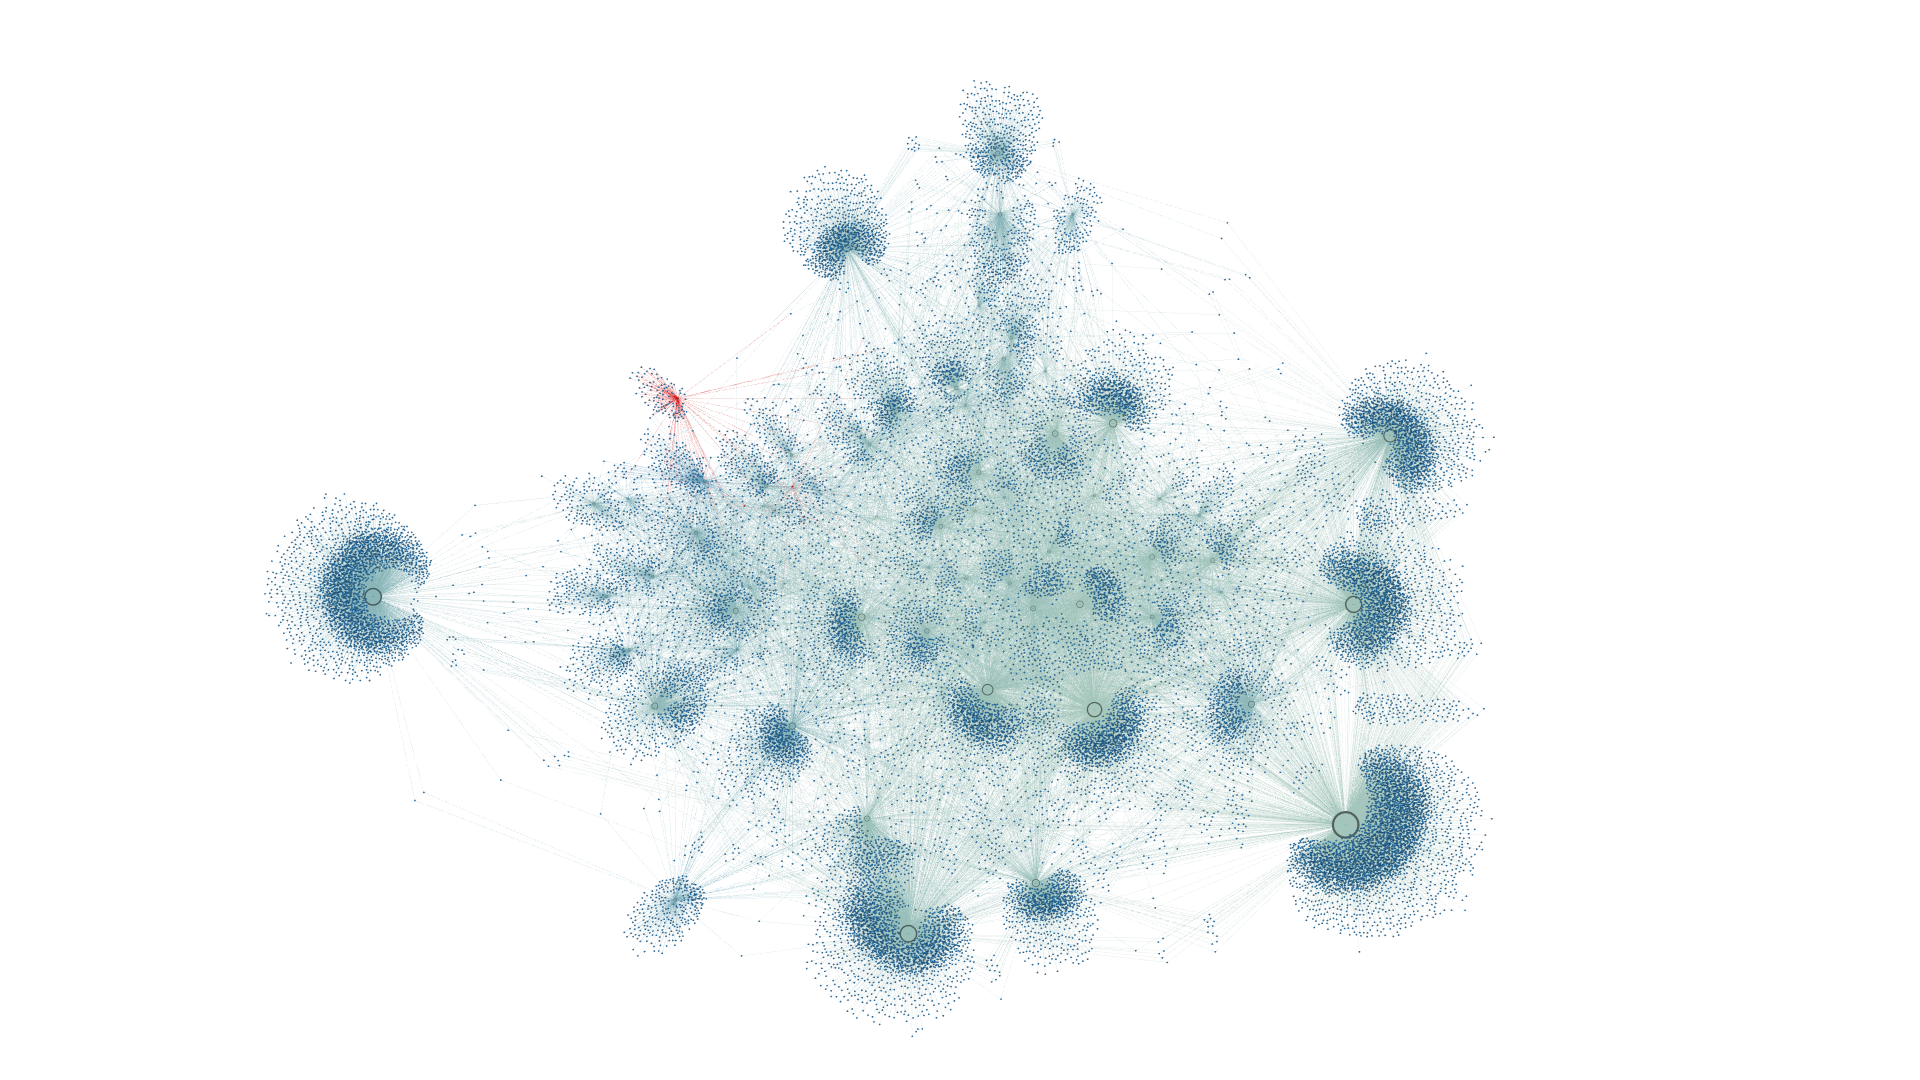
\includegraphics[width=0.9\textwidth]{../Visualizaciones/close}
  \caption{Centralidad de cercanía de la red. Tamaño: \# de nodos, color: valor de centralidad.}
  \label{im4}
\end{figure}


\subsection{Centralidad de excentricidad}

La excentricidad nos indica cómo de central o periférico es un nodo con respecto a sus vecinos según las distancias que los separan. Es decir, un nodo $n_i$ estará en la periferia de la red cuando las distancias a sus vecinos sean muy grandes, y será más central cuando estas distancias sean menores. Esto también es conocido como centralidad de excentricidad, siendo esta la inversa de la máxima distancia geodésica de un nodo con sus vecinos.

\begin{displaymath}
  C_E(i) = \frac{1}{\max_{j \in V(G)/i}d(i,j)}
\end{displaymath}

Los actores con un mayor valor de excentricidad serán los más periféricos, y los de menor, los más centrales.

\begin{table}[H]
\begin{tabular}{l|r}
\textbf{Nodo} & \textbf{Centralidad de} \\
& \textbf{excentricidad} \\
\hline
raymondh & 5.0 \\
python\_vlc & 5.0 \\
fcienciasugr & 4.0 \\
UGRingenieras & 4.0 \\
RealPython & 4.0 \\
dj\_devops & 4.0 \\
OSHLUMH & 4.0 \\
SoyGema & 4.0 \\
cev\_ugr & 4.0 \\
PyConES & 4.0 \\
HackLabAl & 4.0 \\
pythonjaen & 4.0 \\
ETSIIT\_UGR & 4.0 \\
\end{tabular}
\label{eccen}
\caption{Nodos más centrales de la red según la centralidad de excentricidad.}
\end{table}

En la \hyperref[eccen]{Tabla \ref*{eccen}}, podemos ver los nodos con más centrales de la red, es decir, que en un menor número de pasos, llegan a un mayor número de nodos. En la \hyperref[im4]{Figura \ref*{im8}} podemos ver la red, en la que se representa con el tamaño de los nodos el grado que tienen, y en color el grado de centralidad de excentricidad del nodo, siendo más rojo el nodo más central.

\begin{figure}[H]
  \centering
  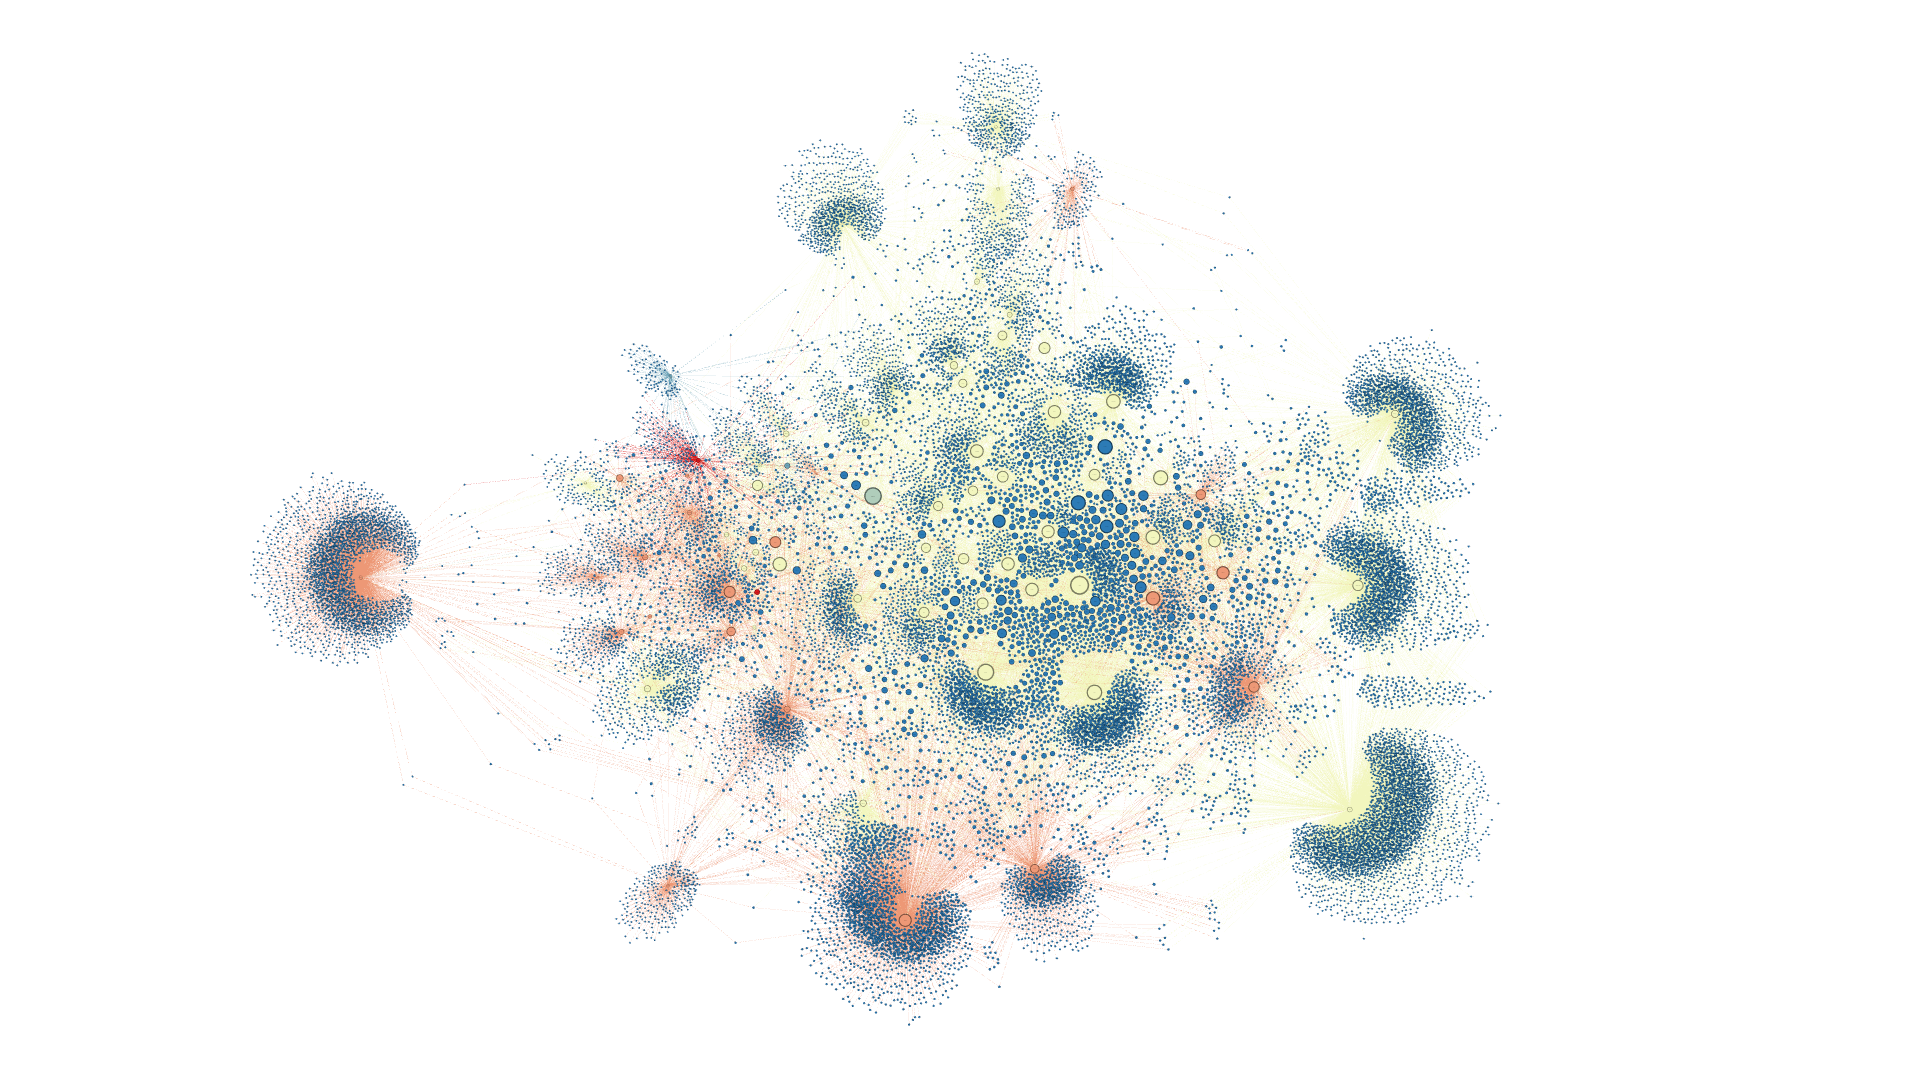
\includegraphics[width=0.9\textwidth]{img/eccen}
  \caption{Centralidad de excentricidad de la red. Tamaño: \# de nodos, color: valor de centralidad.}
  \label{im8}
\end{figure}

\subsection{Intermediación}

La intermediación es una medida que capta la correduría de la información por la estructura de la red. Esta medida da más importancia a los nodos por los que pasen más caminos mínimos por él. Esto se calcula de la siguiente manera:
\begin{displaymath}
  C_B(i) = \sum_{j, k \in V(G)/v}\frac{g_{j,k}(i)}{g_{j,k}}
\end{displaymath}

donde $g_{j,k}$ es el número de caminos mínimos que existen desde el nodo $i$ hasta el nodo $j$ y $g_{j,k}(i)$ es el número de caminos mínimos que pasan por el nodo $i$. Este valor oscilará, al ser una red dirigida, en el intervalo $[0, (g-1)\cdot(g-2)]$.

Esta medida nos permite detectar los nodos conocidos como \textit{\textbf{gatekeepers}}, que son aquellos nodos que actúan como interfaces entre los nodos de distintas comunidades.

En nuestro caso, los actores con mayor valor de intermediación son:

\begin{table}[H]
\begin{tabular}{l|r}
\textbf{Nodo} & \textbf{Valor de centralidad} \\
& \textbf{de intermediación}\\
\hline
python\_granada & 707790.118830 \\
educhip & 292441.166385 \\
HackLabAl & 241062.017686 \\.
PythonEggs & 198534.223102 \\
UGRemprendedora & 178037.331931 \\
renatolrr & 149056.026095 \\
bibliotecaUGR & 137175.695689 \\
python\_es & 135200.241347 \\
OSLUGR & 126351.369941 \\
jjmerelo & 111319.207226 \\
PythonIreland & 104906.281116 \\
OSHLUMH & 99058.494729 \\
Terceranexus6 & 94415.629615 \\
\end{tabular}
\label{between}
\caption{Nodos de la red con mayor valor de centralidad de intermediación o \textit{betweenness centrality}.}
\end{table}

En la \hyperref[between]{Tabla \ref*{between}} podemos ver los actores de la red con mayor valor de intermediación. En ella podemos ver un caso curioso, y es que la propia cuenta de Python Granada tiene el mayor valor de intermediación de la red, es decir, que hace de puerta de enlace con la gran mayoría de comunidades de la red. En la \hyperref[im5]{Figura \ref*{im5}} podemos ver la red, representada igual que antes, el color indica el grado de centralidad y el tamaño el grado del nodo. En esta ocasión, el más central es el nodo de Python Granada, pero tiene un grado tan pequeño en comparación con el resto de la red, que es difícil apreciarlo.
\begin{figure}[H]
  \centering
  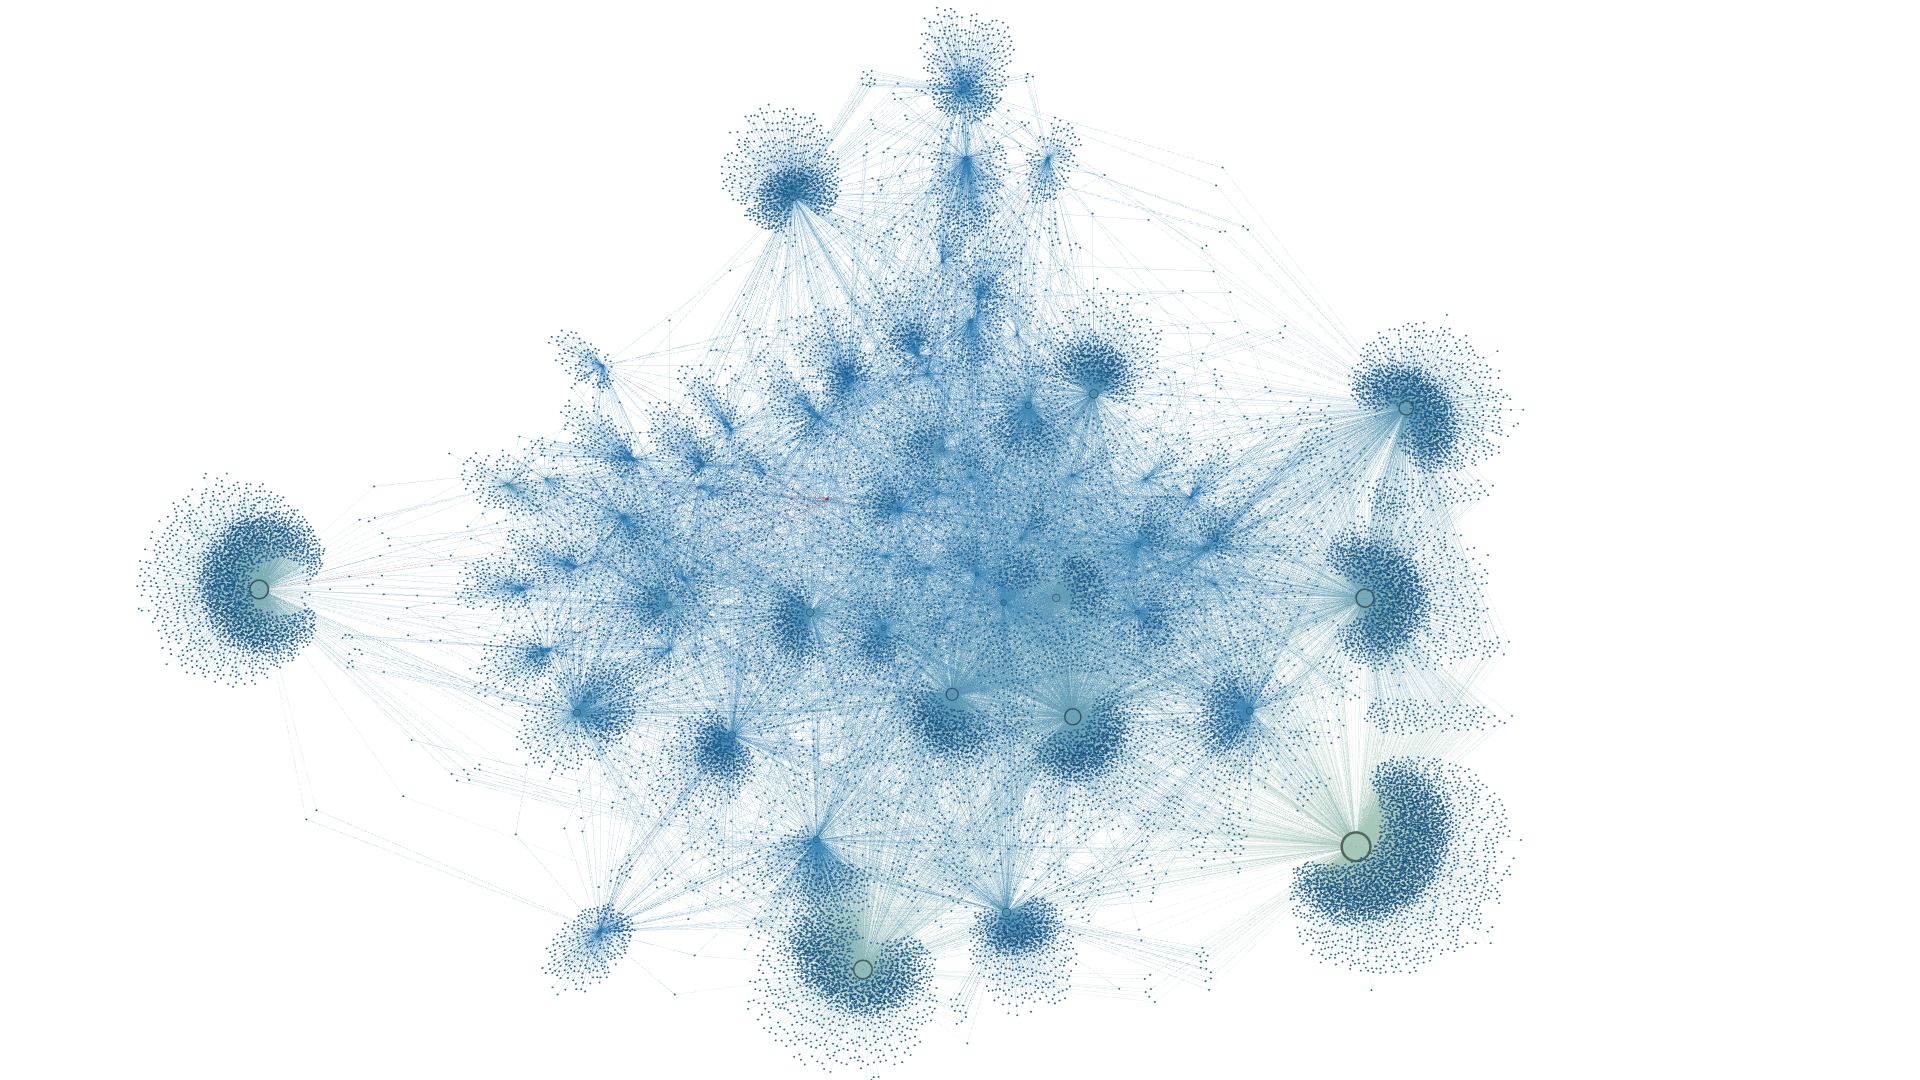
\includegraphics[width=0.9\textwidth]{../Visualizaciones/between}
  \caption{Centralidad de intermediación de la red. Tamaño: \# de nodos, color: valor de centralidad.}
  \label{im5}
\end{figure}

\subsection{Centralidad de vector propio}

La centralidad de vector propio tiene como base la idea de que la centralidad de un nodo depende de cómo de centrales sean sus nodos. Esto se denomina \textit{prominencia}.

Es decir, la importancia o \textbf{ego} de un nodo se define recursivamente de la importancia de sus vecinos o \textbf{alters}. Esta medida es una combinación lineal de los valores de los actores que apunte al nodo $i$, es decir:

\begin{displaymath}
  C_{VP}(i) = a_{1i}\cdot C_{VP}(1) + a_{2i}\cdot C_{VP}(2) + \cdots + a_{ni}\cdot C_{VP}(n)
\end{displaymath}

Para calcular los valores de $C_{VP}$, es necesario construir un sistema de ecuaciones de la forma en la que se define un vector columna $C$ de la forma $C=[C_{VP}(1),C_{VP}(
2),\ldots,C_{VP}(n)]^T$ y este multiplica a la matriz de adyacencia $A$, quedando el sistema de la siguiente manera $$C=A^TC$$.

Resolver este sistema de forma algebraica es demasiado costoso, es por ello por lo que se usa el método iterativo de las potencias, que va iterando poco a poco intentando reducir el error, y dar una buena aproximación.

Esto en definitiva, nos indica qué nodos son los más importantes de la red o tiene un mayor poder de influencia sobre el resto de nodos o actores.

\begin{table}[H]
\begin{tabular}{l|r}
\textbf{Nodo} & \textbf{Centralidad de} \\
& \textbf{vector propio} \\
\hline
OSLUGR & 1.000000 \\
python\_granada & 0.919329 \\
jjmerelo & 0.886500 \\
renatolrr & 0.796691 \\
CanalUGR & 0.784414 \\
delegaETSIIT & 0.777249 \\
fergunet & 0.774187 \\
NuriaStatgirl & 0.761155 \\
Terceranexus6 & 0.744065 \\
python\_es & 0.734991 \\
UGRingenieras & 0.729929 \\
Mrs\_DarkDonado & 0.691699 \\
acanasvargas & 0.689237 \\
\end{tabular}
\label{eigenvec}
\caption{Nodos de la red con mayor valor de centralidad de vector propio o \textit{eigenvector centrality}.}
\end{table}

En la \hyperref[between]{Tabla \ref*{between}} podemos ver los actores que tienen mejor valor de vector propio. En ella podemos ver como la OSL es el nodo de la red con mayor valor de centralidad de vector propio, seguido de Python Granada y del profesor Juan Julía Merelo, como los más influyentes de la red. En la \hyperref[im6]{Figura \ref*{im6}} podemos ver la red, donde destacan los nodos de color rojo como los nodos con mayor centralidad de vector propio. En ella podemos ver cómo estos nodos son en su mayoría los más influyentes pertenecientes a la zona central de la red.

\begin{figure}[H]
  \centering
  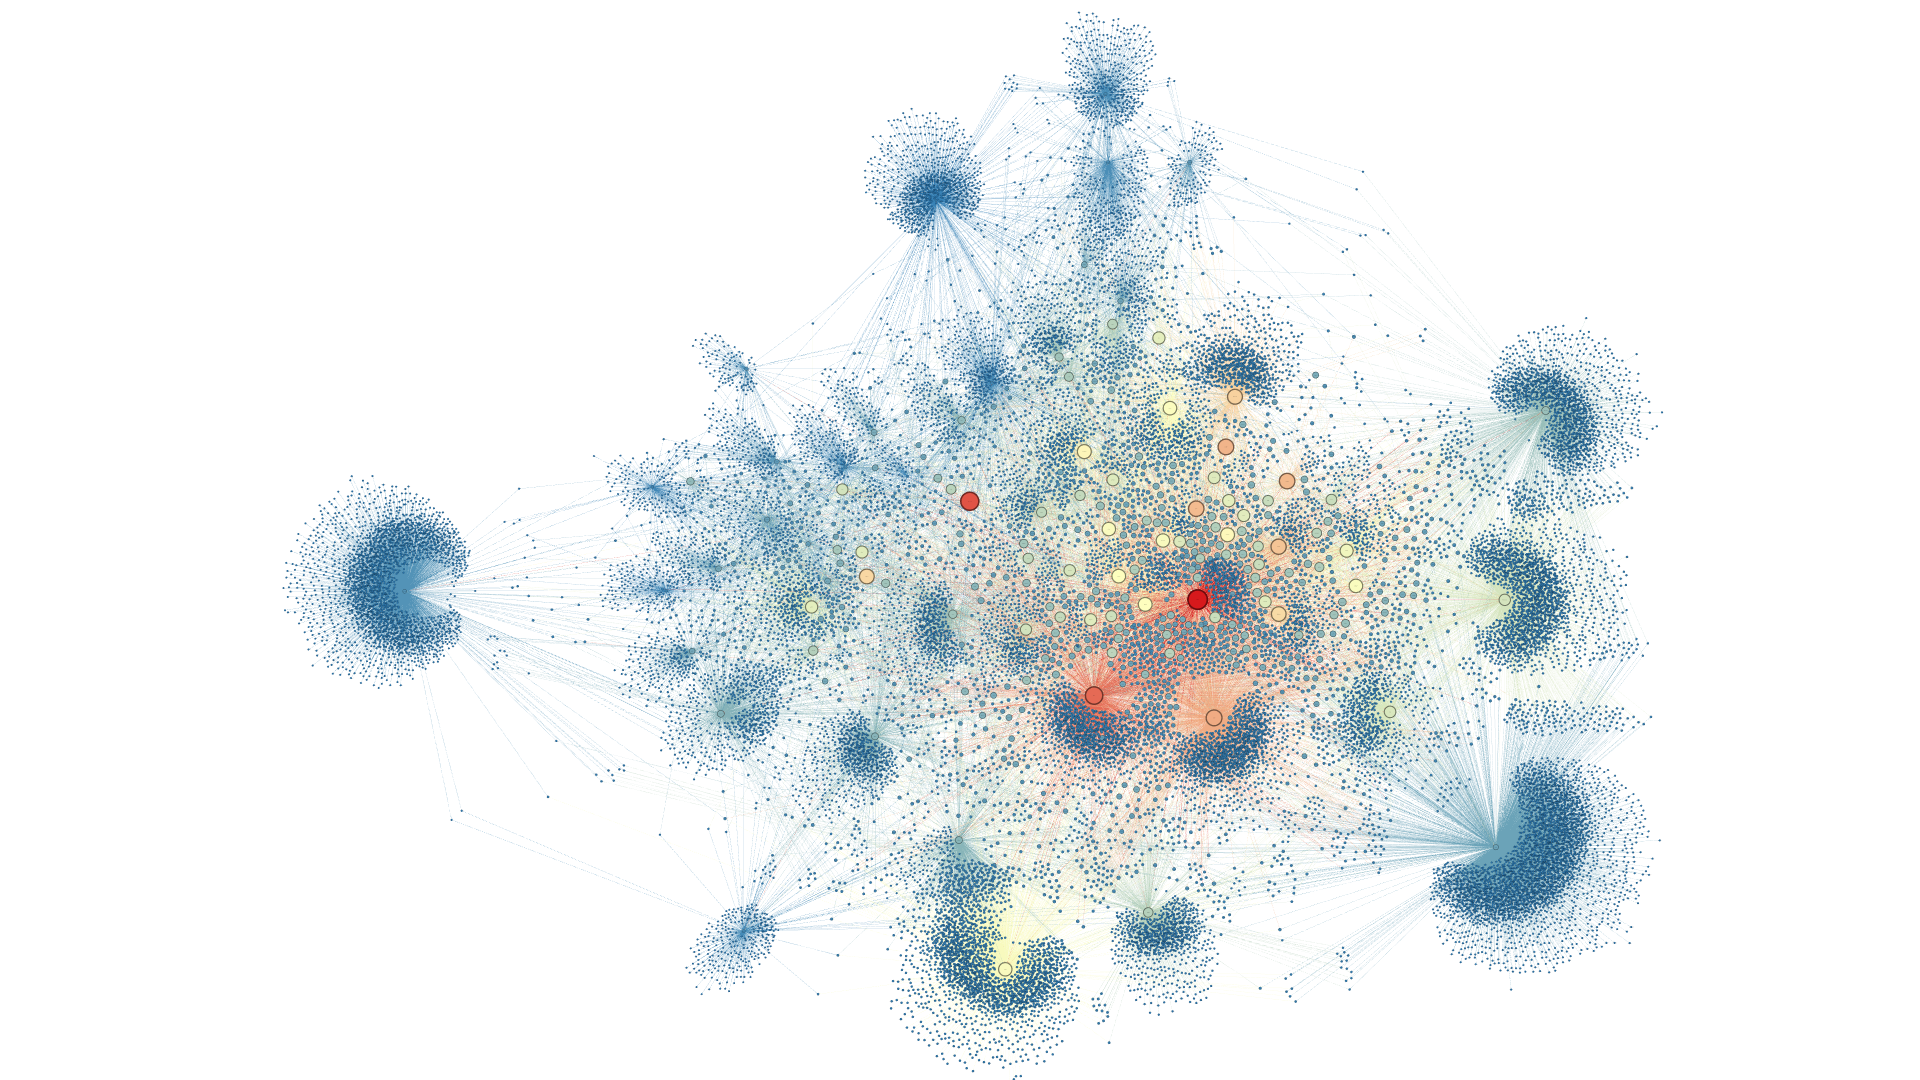
\includegraphics[width=0.9\textwidth]{../Visualizaciones/eigenvec}
  \caption{Centralidad de vector propio de la red. Tamaño: \# de nodos, color: valor de centralidad.}
  \label{im6}
\end{figure}

\section{Detección de comunidades}

Antes de empezar a detectar las comunidades que existen en una red, es interesante ver qué grado de modularidad tiene. Como hemos visto en la \hyperref[estadisticas]{Tabla \ref*{estadisticas}}, esta red tiene un alto grado de modularidad, por lo que presenta dentro una estructura modular muy fuerte, lo que nos permite hacer una buena detección de comunidades.

Para esta tarea, existen varios métodos:

\begin{enumerate}[$\bullet$]
  \item \textbf{Método de Lovaina}.
  \item \textbf{Método de clustering estocástico}.
  \item \textbf{Método de clustering jerárquico aglomerativo estocástico}.
\end{enumerate}

A continuación, vamos a ver uno por uno los distintos métodos.

\subsection{Método de Lovaina}

Este es el método que trae Gephi implementado de base. Es un método de clustering jerárquico muy eficiente capaz de manejar un gran número de nodos. Es un algoritmo con un enfoque greedy que va optimizando de manera local la medida de la modularidad hasta que no se produce mejora.

Tiene dos partes, una de optimización en la que, mediante un método de ascensión de colinas trata de mover los nodos entre comunidades, siempre y cuando el valor de $Q$ vaya mejorando; y otro de agregación, en el que va generando nodos de gran tamaño a base de juntar en un mismo nodo las comunidades detectadas.

En la \hyperref[im7]{Figura \ref*{im7}}, podemos ver la partición que ha hecho el método de Lovaina, junto con una visualización de la red por colores. Esta partición ha conseguido un valor de $Q = 0.743$.

\begin{figure}[H]
  \centering
  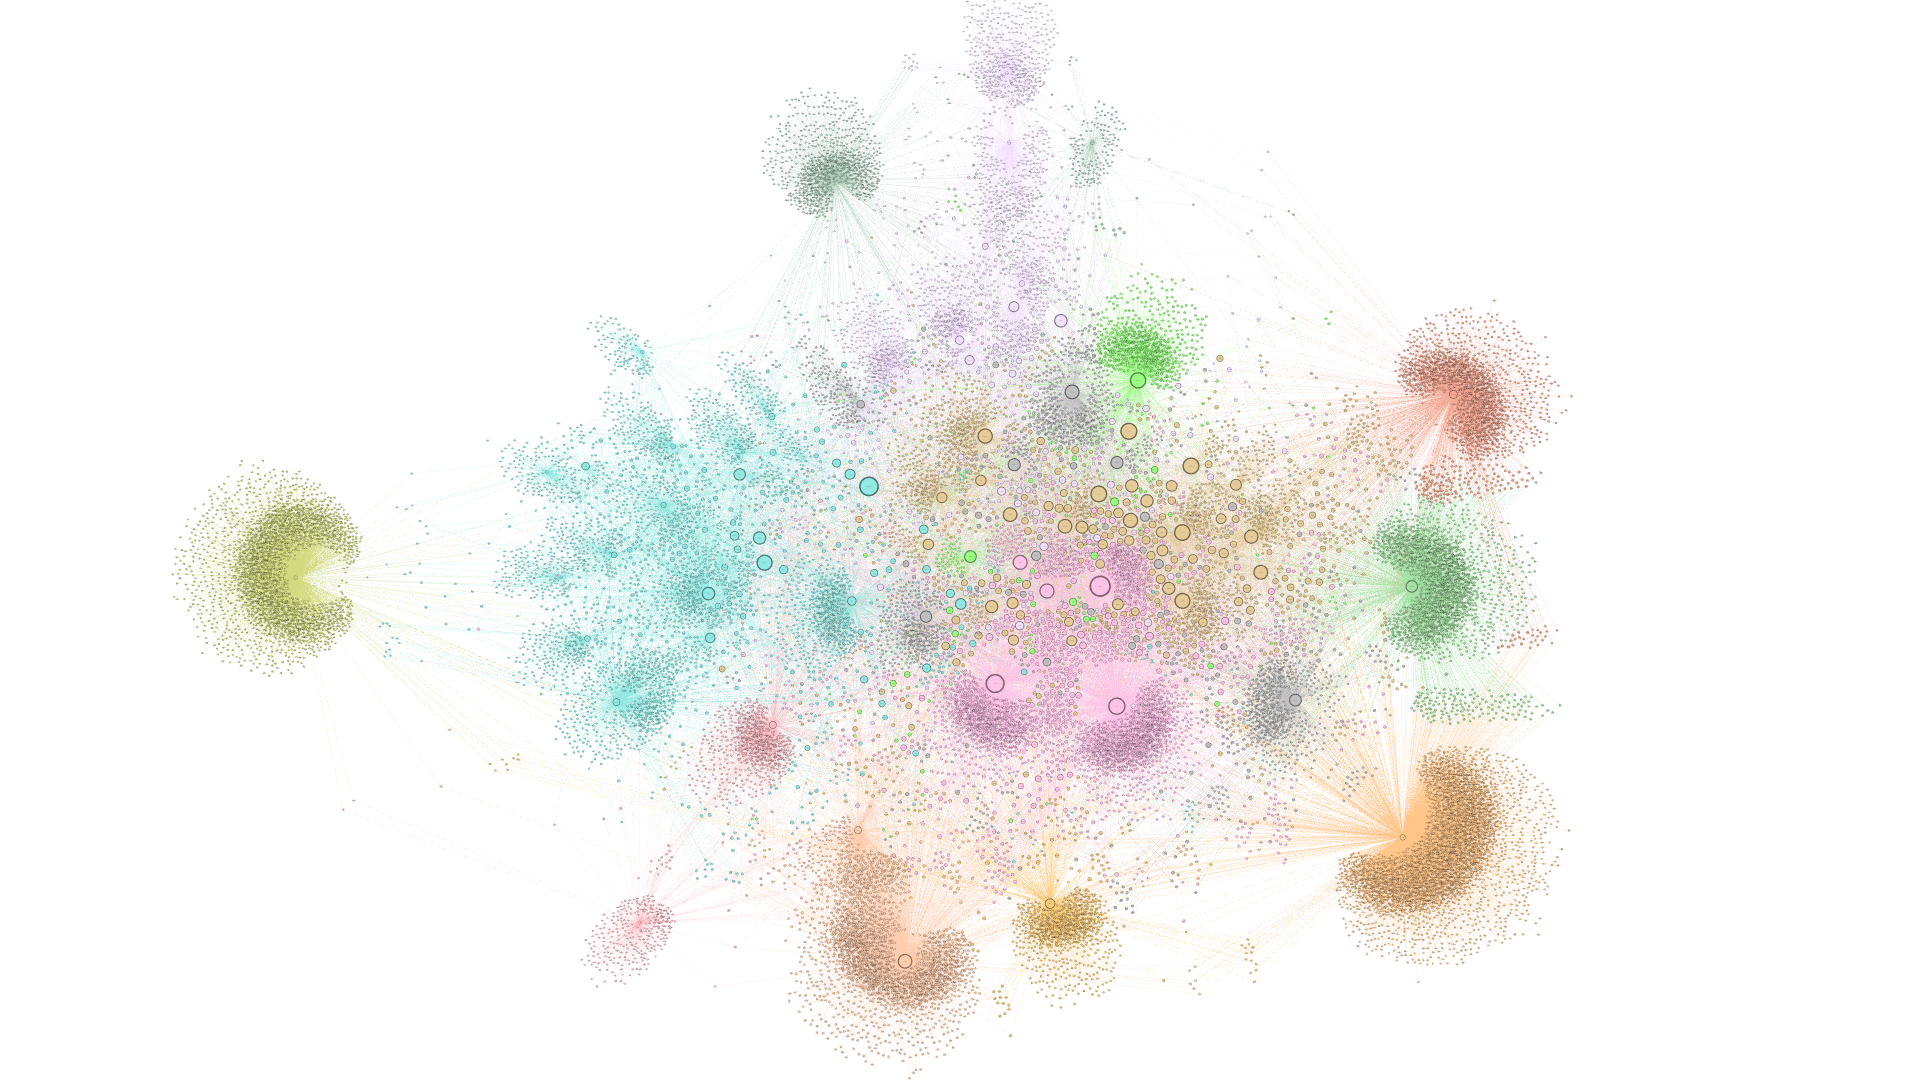
\includegraphics[width=0.9\textwidth]{img/community}
  \caption{Comunidades detectadas en la red.}
  \label{im7}
\end{figure}

A continuación, en la \hyperref[com_lov]{Tabla \ref*{com_lov}} podemos ver las comunidades que ha detectado, según la clasificación por colores y el porcentaje que representa.

\begin{table}
  \begin{tabular}{l|c|c}
    Comunidad & Color & Porcentaje \\
    \hline
    Comunidad de amigos de \textit{educhip} & \cellcolor[RGB]{255, 186, 116} & 12.8\%\\
    Comunidades de Python & \cellcolor[RGB]{116,209,255} & 12.69\%\\
    OSL Granada & \cellcolor[RGB]{255, 153, 254} & 11.41\%\\
    Comunidad de amigos de \textit{PythonEggs} & \cellcolor[RGB]{200, 217, 117} & 9.01\%\\
    Comunidad de desarrolladores de Almería & \cellcolor[RGB]{255,207,173} & 8.12\%\\
    Doble grado IM & \cellcolor[RGB]{243,225,255} & 7.36\% \\
    Comunidad de emprendedores & \cellcolor[RGB]{138, 213, 168} & \\
    UGR emprendedora & \cellcolor[RGB]{138, 213, 168} & 6.82\%\\
    Grupos y alumnos de la UGR & \cellcolor[RGB]{213, 184, 138} & 6.42\%\\
    Biblioteca de la UGR & \cellcolor[RGB]{244,167,123} & 5.89\%\\
    Comunidad externa de Córdoba & \cellcolor[RGB]{133, 203, 195} & 3.43\%\\
    Ponentes de PyConES16 & \cellcolor[RGB]{255, 163, 163} &  3.36\%\\
    OSHLUMH & \cellcolor[RGB]{246, 197, 124} &  3.08\%\\
    Comunidad de Campus &\cellcolor[RGB]{153,255,128} & \\
    UGRIngenieras, Terceranexus... & \cellcolor[RGB]{153,255,128} & 2.85\%\\
  \end{tabular}
  \label{com_lov}
  \caption{Comunidades más relevantes de la red y su porcentaje de las 55 encontradas.}
\end{table}

\subsection{Método de clustering estocástico y Clustering jerárquico estocástico}

Estos métodos están disponibles en el framework \textit{Graph-tool}\cite{peixoto_graph-tool_2014}. Ambos métodos van aglomerando nodos formando comunidades de nodos de forma aleatoria para calcular las comunidades. Aquellos nodos que pertenezcan al mismo grupo, tendrán la misma probabilidad de estar conectados, siendo estos los que acaben formando la comunidad. De esta forma, tras varias iteraciones, va formando poco a poco las comunidades obteniendo un mejor valor de modularidad.

La versión jerárquica se utiliza para redes de gran tamaño ya que el algoritmo se centra en detectar comunidades a distintas escalas de la red para luego ir superponiéndolas para detectar comunidades de mayor tamaño y de forma más eficiente. Es por esto por lo que en este caso, vamos a utilizar la versión jerárquica, ya que los tiempos de cómputo de la versión normal, para el tamaño de la red son de horas, mientras que la versión jerárquica son unos pocos segundos.

Con esta versión del algoritmo conseguimos la siguiente distribución de comunidades, que queda representada en la \hyperref[im9]{Figura \ref*{im9}}.

\begin{figure}[H]
  \centering
  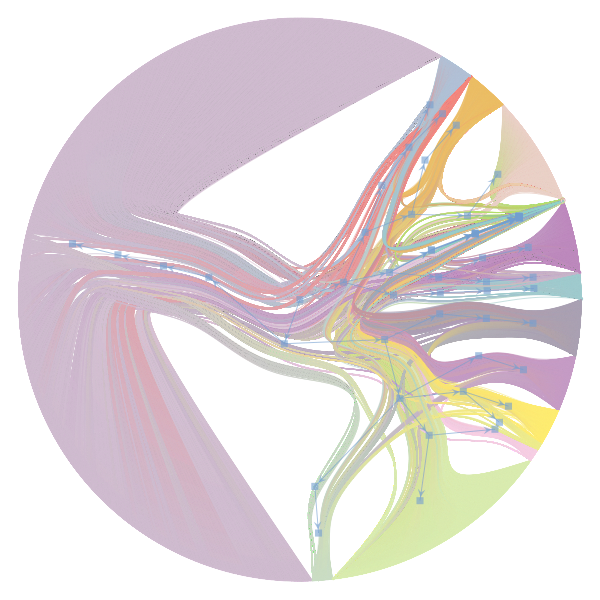
\includegraphics[width=0.6\textwidth]{img/stoc}
  \caption{Partición de nodos para el Nested Stochastic Block Model.}
  \label{im9}
\end{figure}

\begin{table}
\begin{tabular}{l|r}
Id comunidad & \%\\
\hline
0 & 0.044738 \\
1 & 1.511520 \\
2 & 2.019621 \\
3 & 0.012782 \\
4 & 0.006391 \\
5 & 0.057521 \\
6 & 0.003196 \\
7 & 3.221168 \\
8 & 0.009587 \\
9 & 0.015978 \\
10 & 0.009587 \\
11 & 2.390311 \\
12 & 0.015978 \\
13 & 0.006391 \\
14 & 6.375228 \\
15 & 0.025565 \\
16 & 0.741380 \\
17 & 0.009587 \\
18 & 0.006391 \\
19 & 59.048349 \\
20 & 3.240341 \\
21 & 4.112741 \\
22 & 0.006391 \\
23 & 1.156808 \\
24 & 13.443901 \\
25 & 0.389864 \\
26 & 2.118685 \\
\end{tabular}
\label{coms3}
\caption{Comunidades encontradas por el Nested Stochastic Block Model:  27}
\end{table}

Como vemos, este método frente al de Lovaina, ha encontrado menos comunidades, pero, ha encontrado a su vez comunidades más grandes, encontrando una que representa aproximadamente el 60\% de la red, como se ve en la \hyperref[im9]{Figura \ref*{im9}}.

\section{Estudio para la mejora de la difusión}

Una vez estudiados todos estos datos, podemos proceder a estudiar la red más deteninamente para mejorar la difusión. Partimos de que la red es libre de escala, lo que nos indica que, es muy vulnerable a ataques dirigidos por la existencia de hubs, que existen caminos de corta longitud, y sabemos cuáles son los nodos más centrales de cada longitud.

El proceso que vamos a realizar es similar a un proceso de marketing viral, en el que se intenta que una noticia llegue a al mayor número de nodos posible, cuando no es posible aumentar la recompensa que ofrece el producto, es decir, mayor calidad por el mismo precio o similares. En este caso, nosotros no podemos aumentar la recompensa, ya que no estamos ofreciendo ningún producto y solo queremos llegar a un mayor número de personas.

En este proceso, se recompensa o se influye sobre un pequeño número de nodos conocidos como las semillas, que al tener más influencia sobre el resto de nodos, son capaces de viralizar el producto. Estos nodos pueden ser los hubs de la red, ya que viralizan la opinión al tener un gran número de conexiones con otros actores de la red.

Pero, estos no tienen por qué ser los más influyentes de la red. En secciones anteriores hemos visto cómo la centralidad o importancia de un nodo, cambia según el enfoque que le demos. Es por esto, por lo que los hubs son importantes en la red, eso es cierto, pero puede ser que un nodo que esté muy cercano a un hub también sea importante, o más aún, un nodo que haga de gatekeeper entre dos comunidades diferentes, pudiendo hacer que si la opinión del producto se está propagando en una comunidad $A$, esta opinión no llegue a una comunidad $B$ y viceversa.

Es por esto, por lo que nos vamos a centrar en las medidas de centralidad de vector propio, la centralidad de cercanía, y la de intermediación en la red, para intentar ver si es posible o no que se produzca una \textbf{propagación en cascada}.

 Hay que tener en cuenta que, para un estudio más profundo de la viralidad de una publicación o marketing viral, hay que tener más variables, pero en este caso, como el producto son charlas o eventos, y el beneficio que puede producir a un actor $n_i$ no es más que conocimiento, la influencia de ventas no existe, el coste tampoco porque son gratuitas, además de otros valores que se utilizan en marketing, por lo que buscaremos aquellos nodos más influyentes de la red.

Para empezar el análisis, eliminaremos el nodo de Python Granada, para que la red deje de ser egocéntrica, y podamos centrarnos mejor en cada comunidad. Si nos fijamos en las comundidades que hemos detectado en la \hyperref[com_lov]{Tabla \ref*{com_lov}}, vamos a ir haciendo un análisis por comunidades, poniendo el ``\textit{top 3}'' más importante de cada comunidad, según los valores de centralidad de vector propio, intermediación, cercanía y excentricidad:

\begin{enumerate}[$\bullet$]
  \item \textbf{Comunidad de amigos de \textit{educhip}:}
  \begin{enumerate}[---]
    \item \textit{Centralidad de Cercanía}:
    \begin{enumerate}
      \item educhip.
    \end{enumerate}
    \item \textit{Centralidad de Excentricidad}:
    \begin{enumerate}
      \item educhip.
    \end{enumerate}
    \item \textit{Centralidad de Intermediación}:
    \begin{enumerate}
      \item educhip.
    \end{enumerate}
    \item \textit{Centralidad de Vector Propio}:
    \begin{enumerate}
      \item educhip.
    \end{enumerate}
  \end{enumerate}
  Esta comunidad, aunque sea la que representa un mayor porcentaje en la red, todos son dos que cuelgan de él, sin interacción en la red, por lo que para poder llegar a esta comunidad es imprescindible que la publicación llegue a \textbf{educhip}.
  \item \textbf{Comunidades de Python:}
  \begin{enumerate}[---]
    \item \textit{Centralidad de Cercanía}:
    \begin{enumerate}
      \item minrk.
      \item SciPyTip.
      \item pydatasci.
    \end{enumerate}
    \item \textit{Centralidad de Excentricidad}:
    \begin{enumerate}
      \item python\_vlc.
      \item raymondh.
      \item Pybonacci.
    \end{enumerate}
    \item \textit{Centralidad de Intermediación}:
    \begin{enumerate}
      \item python\_es.
      \item PythonIreland.
      \item Pybonacci.
    \end{enumerate}
    \item \textit{Centralidad de Vector Propio}:
    \begin{enumerate}
      \item python\_es.
      \item Pybonacci.
      \item PyConEs.
    \end{enumerate}
  \end{enumerate}
  En este caso, los nodos principales de la red barían mucho entre sí, aunque, destacan en esta red las cuentas de \textbf{Pybonacci}, por su centralidad y su capacidad de correduría de las noticias y \textbf{python\_es}, la cuenta oficial de la asociación de Python España, ya que se posiciona como la que más capacidad tiene para mover una noticia, y la más importante de la red como indica su capacidad de vector propio, es por eso, que para producir un efecto en cascada es interesante tener a estos dos nodos en cuenta, ya que son capaces de difundir un evento o noticia a través de todas las comunidades de Python españolas, llegando incluso a cruzar el océano llegando a cuentas como \textit{argenpython} (la cuenta de Python Argentina), \textit{Python Ireland}...
  \item \textbf{OSL Granada:}
  \begin{enumerate}[---]
    \item \textit{Centralidad de Cercanía}:
    \begin{enumerate}
      \item renatolrr.
      \item OSLUGR.
      \item jjmerelo.
    \end{enumerate}
    \item \textit{Centralidad de Excentricidad}:
    \begin{enumerate}
      \item renatolrr.
      \item OSLUGR.
      \item jjmerelo.
    \end{enumerate}
    \item \textit{Centralidad de Intermediación}:
    \begin{enumerate}
      \item renatolrr.
      \item OSLUGR.
      \item jjmerelo.
    \end{enumerate}
    \item \textit{Centralidad de Vector Propio}:
    \begin{enumerate}
      \item OSLUGR.
      \item jjmerelo.
      \item renatolrr.
    \end{enumerate}
  \end{enumerate}
  En la red que forma la OSL de la Universidad de Granada, vemos que los principales actores de la red son sin duda \textbf{renatolrr}, \textbf{OSLUGR} y \textbf{jjmerelo}. Por lo tanto, no hay duda de que para difundir un evento por esta comunidad, son los actores principales de la red, aunque si usamos el conocimiento real que disponemos antes de hacer el estudio, en este caso, con tan solo influir sobre el nodo de la OSL, llegaremos a toda la red, por lo que nos ahorraríamos bastante en el caso de que hubiera que pagar dinero.
  \item \textbf{Comunidad de amigos de \textit{PythonEggs}:}
  \begin{enumerate}[---]
    \item \textit{Centralidad de Cercanía}:
    \begin{enumerate}
      \item PythonEggs.
    \end{enumerate}
    \item \textit{Centralidad de Excentricidad}:
    \begin{enumerate}
      \item PythonEggs.
    \end{enumerate}
    \item \textit{Centralidad de Intermediación}:
    \begin{enumerate}
      \item PythonEggs.
    \end{enumerate}
    \item \textit{Centralidad de Vector Propio}:
    \begin{enumerate}
      \item PythonEggs.
      \item pe\_braun.
      \item tecno\_instante.
    \end{enumerate}
  \end{enumerate}
  En este caso, sucede algo muy similar a lo que pasaba con la primera comunidad, pero la diferencia está en que al no estar tan aislada, la centralidad de vector propio varía, pero en definitiva, el nodo que se influiría para producir un efecto en cascada es sin duda \textbf{PythonEggs}, por las propiedades que tiene este nodo, en caso de que quisiéramos llevar la noticia o evento a comunidades extranjeras.
  \item \textbf{Comunidad de desarrolladores de Almería:}
  \begin{enumerate}[---]
    \item \textit{Centralidad de Cercanía}:
    \begin{enumerate}
      \item GDGAlmeria.
      \item HackLabAl.
    \end{enumerate}
    \item \textit{Centralidad de Excentricidad}:
    \begin{enumerate}
      \item HackLabAl.
      \item GDGAlmeria.
    \end{enumerate}
    \item \textit{Centralidad de Intermediación}:
    \begin{enumerate}
      \item HackLabAl.
      \item GDGAlmeria.
    \end{enumerate}
    \item \textit{Centralidad de Vector Propio}:
    \begin{enumerate}
      \item HackLabAl.
      \item GDGAlmeria.
      \item antonio1010mr.
    \end{enumerate}
  \end{enumerate}
  En esta comunidad, sin duda para producir el efecto cascada, los nodos relevantes son \textbf{HackLabAl} y \textbf{GDGAlmeria} que son sin duda los más importantes, y el nodo \textit{antonio1010mr}, su valor de centralidad de vector propio es irrelevante en comparación con el de los otros dos nodos.
  \item \textbf{Doble grado IM:}
  \begin{enumerate}[---]
    \item \textit{Centralidad de Cercanía}:
    \begin{enumerate}
      \item fdavidcl.
      \item xiroux.
      \item libreim\_.
    \end{enumerate}
    \item \textit{Centralidad de Excentricidad}:
    \begin{enumerate}
      \item fdavidcl.
      \item xiroux.
      \item libreim\_.
    \end{enumerate}
    \item \textit{Centralidad de Intermediación}:
    \begin{enumerate}
      \item Pacoluque95.
      \item libreim\_.
      \item xiroux.
    \end{enumerate}
    \item \textit{Centralidad de Vector Propio}:
    \begin{enumerate}
      \item libreim\_.
      \item fdavidcl.
      \item mroman42.
    \end{enumerate}
  \end{enumerate}

  En esta comunidad, los más influyentos son sin duda el nodo de \textbf{fdavidcl}, \textbf{xiroux} y \textbf{libreim}\_. También es interesante interesarse por \textbf{mroman42}, pero con los otros tres nodos, también llegaríamos a él, pero siguiendo la estructura de la red, puede que hubiera partes de la comunidad que se quedaran aisladas.

  \item \textbf{Comunidad de emprendedores y UGR emprendedora:}
  \begin{enumerate}[---]
    \item \textit{Centralidad de Cercanía}:
    \begin{enumerate}
      \item UGRemprendedora.
    \end{enumerate}
    \item \textit{Centralidad de Excentricidad}:
    \begin{enumerate}
      \item UGRemprendedora.
    \end{enumerate}
    \item \textit{Centralidad de Intermediación}:
    \begin{enumerate}
      \item UGRemprendedora.
    \end{enumerate}
    \item \textit{Centralidad de Vector Propio}:
    \begin{enumerate}
      \item UGRemprendedora.
    \end{enumerate}
  \end{enumerate}
  En este caso, sucede el mismo caso que en la primera comunidad. Todos los nodos cuelgan prácticamente del nodo de \textbf{UGRemprendedora}, luego sin duda para expandir el efecto cascada por esta comunidad, deberíamos influenciar al nodo de UGRemprendedora.
  \item \textbf{Grupos y alumnos de la UGR:}
  \begin{enumerate}[---]
    \item \textit{Centralidad de Cercanía}:
    \begin{enumerate}
      \item brau\_vl.
      \item DatosUGR.
      \item NuriaStatgirl.
    \end{enumerate}
    \item \textit{Centralidad de Excentricidad}:
    \begin{enumerate}
      \item ETSIIT\_UGR.
      \item fcienciasugr.
      \item UGRingenieras.
    \end{enumerate}
    \item \textit{Centralidad de Intermediación}:
    \begin{enumerate}
      \item Mrs\_Darkdonado.
      \item geekandtechgirl.
      \item DatosUGR.
    \end{enumerate}
    \item \textit{Centralidad de Vector Propio}:
    \begin{enumerate}
      \item CanalUGR.
      \item delegaETSIIT.
      \item fergunet.
    \end{enumerate}
  \end{enumerate}
  En este caso, existe una gran variedad de nodos, no quedando muy claro cuál sería el más relevante para producir un efecto cascada, pero si usamos la información global de la red, vemos que muchos de estos nodos están conectados a la comunidad de la OSL, las comunidades de Python (Python España, Python Granada, Pybonacci...) por lo que podrían llegarle las corredurías muy fácilmente por otro camino, así que, para llegar a más personas produciendo un efecto cascada, los más interesantes serían los nodos de \textbf{geekandtechgirl}, \textbf{delegaETSIIT}, \textbf{ETSII\_UGR} y sobretodo, \textbf{CanalUGR}.
  \item \textbf{Biblioteca de la UGR:}
  \begin{enumerate}[---]
    \item \textit{Centralidad de Cercanía}:
    \begin{enumerate}
      \item bibliotecaUGR.
    \end{enumerate}
    \item \textit{Centralidad de Excentricidad}:
    \begin{enumerate}
      \item bibliotecaUGR.
    \end{enumerate}
    \item \textit{Centralidad de Intermediación}:
    \begin{enumerate}
      \item bibliotecaUGR.
    \end{enumerate}
    \item \textit{Centralidad de Vector Propio}:
    \begin{enumerate}
      \item bibliotecaUGR.
    \end{enumerate}
  \end{enumerate}
  Similar al primer caso.
  \item \textbf{Comunidad externa de Córdoba:}
  \begin{enumerate}[---]
    \item \textit{Centralidad de Cercanía}:
    \begin{enumerate}
      \item sergiormb.
      \item JotaEntrena.
    \end{enumerate}
    \item \textit{Centralidad de Excentricidad}:
    \begin{enumerate}
      \item JotaEntrena.
      \item sergiormb.
    \end{enumerate}
    \item \textit{Centralidad de Intermediación}:
    \begin{enumerate}
      \item sergiormb.
      \item JotaEntrena.
    \end{enumerate}
    \item \textit{Centralidad de Vector Propio}:
    \begin{enumerate}
      \item SuMalevolencia\_. 
      \item granadagaming.
      \item elmundotoday.
    \end{enumerate}
  \end{enumerate}
  En este caso, los más interesantes serían los nodos \textbf{SuMalevolencia\_}, \textbf{granadagaming} y \textbf{sergiormb}, aunque esta pequeña comunidad, ya cuelga de comunidades como los grupos y los alumnos de la UGR, el doble grado, etc.
  \item \textbf{Ponentes de PyConES16:}
  \begin{enumerate}[---]
    \item \textit{Centralidad de Cercanía}:
    \begin{enumerate}
      \item SoyGema.
      \item carmeartigas.
    \end{enumerate}
    \item \textit{Centralidad de Excentricidad}:
    \begin{enumerate}
      \item SoyGema.
      \item carmeartigas.
    \end{enumerate}
    \item \textit{Centralidad de Intermediación}:
    \begin{enumerate}
      \item SoyGema.
      \item carmeartigas.
    \end{enumerate}
    \item \textit{Centralidad de Vector Propio}:
    \begin{enumerate}
      \item SoyGema.
      \item juanrrcc.
      \item oculus.
    \end{enumerate}
  \end{enumerate}
  En esta red, la más importante es \textbf{SoyGema}, ponente en la PyconES16. Este nodo es el más influyente de la red, pero, ya estamos hablando de comunidades muy pequeñas, y con una alta relación con las comunidades de Python, así que quizá fuera interesante influenciar a este nodo, ya que fuera de la red, Gema es un hub de muy gran tamaño y con mucha relevancia social.
\end{enumerate}

Esto es un estudio mucho más fino que si realizamos una partición por comunidades mucho más grande como la que se ve en la \hyperref[im11]{Figura \ref*{im11}}, pero si realizamos un análisis más general, podríamos cubrir casi toda la red si influenciamos los nodos de la OSL y CanalUGR, para la comunidad de Granada (rosa), y los nodos de python\_es y Pybonacci para la red de comunidades de Python (azul), ahorrando muchos más costes (si los hubiera) que antes, y ahorrándo el spam que podríamos producir si influenciamos a demasiados.

\begin{figure}[H]
  \centering
  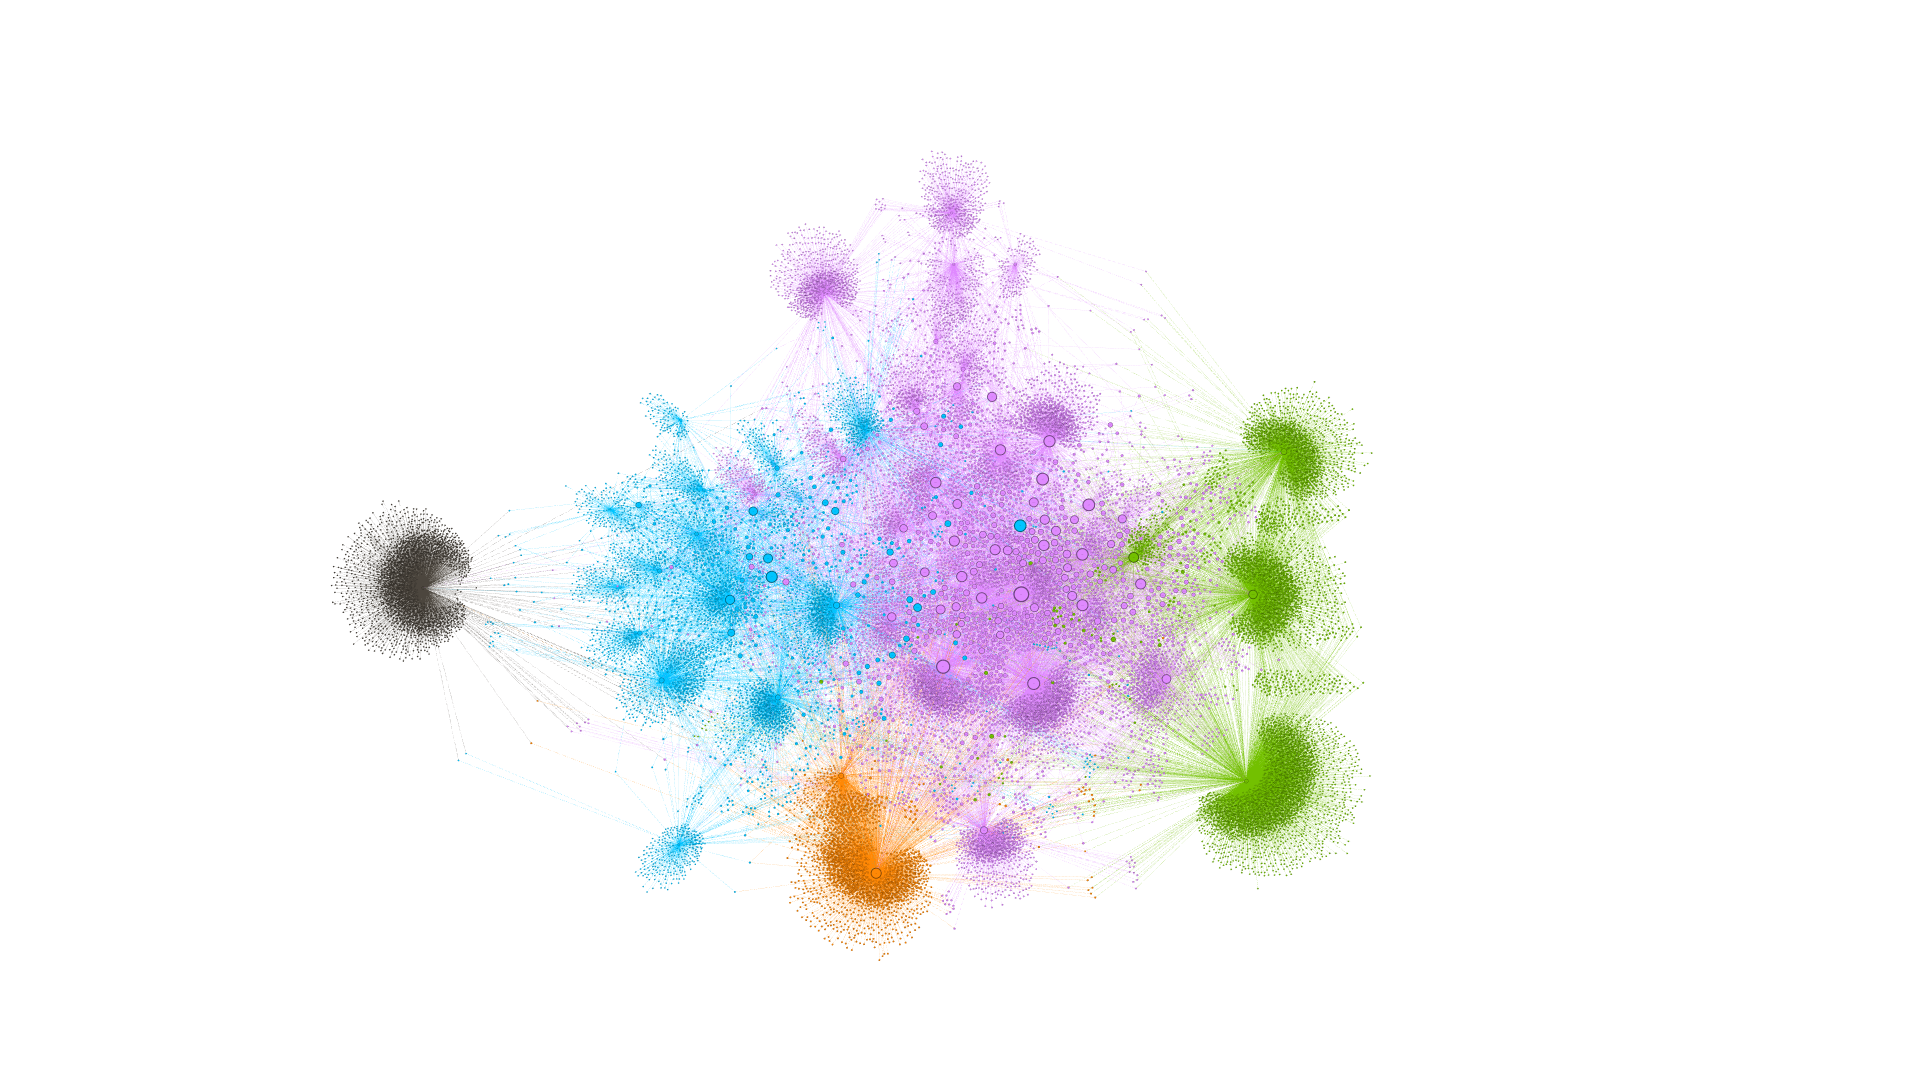
\includegraphics[width=0.9\textwidth]{img/comBig}
  \caption{Partición de nodos más general.}
  \label{im11}
\end{figure}

\section{Conclusiones finales}

En definitiva, los datos extraídos han sido útiles para el estudio realizado, mostrándo cosas que concuerdan con la realidad, con el conocimiento que tenía a priori, y muy útiles para el descubrimiento del conocimiento, haciendo uso de la estructura de grafo. 

También, gracias al estudio de la red, se puede comprobar cómo los nodos varían de importancia según la medida de centralidad que estemos usando, y como nodos que, por la distribución de la red o el algoritmo de \textit{layout}, pueden parecer nodos muy excéntricos, pero en realidad, son nodos muy centrales en la red y que manejan mucho el flujo de información que sucede en esta, siendo el caso de \textit{minrk}, que es uno de los nodos con más valor de cercanía en la red.

\bibliography{citations} %archivo citas.bib que contiene las entradas 
\bibliographystyle{plain} % hay varias formas de citar

\end{document}
